\documentclass[12pt,a4paper,oneside]{report}

% ── Packages ──
\usepackage[utf8]{inputenc}
\usepackage[T1]{fontenc}
\usepackage{geometry}
\geometry{left=2.5cm,right=2.5cm,top=2.5cm,bottom=2.5cm}
\usepackage{setspace}
\onehalfspacing
\usepackage{graphicx}
\usepackage{booktabs}
\usepackage{amsmath}
\usepackage{amssymb}
\usepackage{hyperref}
\hypersetup{
    colorlinks=true,
    linkcolor=black,
    citecolor=black,
    urlcolor=blue
}
\usepackage{caption}
\usepackage{subcaption}
\usepackage{float}
\usepackage{fancyhdr}

% ── Header / Footer ──
\setlength{\headheight}{14.5pt}
\pagestyle{fancy}
\fancyhf{}
\rhead{\thepage}
\lhead{\leftmark}

% ── Title Page Info ──
\title{
    \vspace*{2cm}
    \textbf{A Deep Learning-Based Non-Destructive Testing (NDT) Approach for\\[4pt]
    Brick Quality Assessment via Mel-Spectrogram Analysis}
}
\author{
    Md. Ashraful Islam\\[6pt]
    \small Roll: 22102004\\[6pt]
    \small Department of Computer Science and Engineering\\[6pt]
    \small Jatiya Kabi Kazi Nazrul Islam University
}
\date{\today}

% ═══════════════════════════════════════════════
\begin{document}

% ── Title Page ──
\maketitle
\thispagestyle{empty}
\newpage

% ── Declaration ──
\chapter*{Declaration}
\addcontentsline{toc}{chapter}{Declaration}

I hereby declare that the work presented in this interim thesis report, titled
\textit{``A Deep Learning-Based Non-Destructive Testing (NDT) Approach for
Brick Quality Assessment via Mel-Spectrogram Analysis''}, is my own original
work. This report documents the preparatory research, literature review,
dataset analysis, and methodology planning completed during the current
semester as part of the thesis course CSE 400(A).

To the best of my knowledge, this work contains no material previously
published or written by another person, except where due reference has been
made in the text. This work has not been submitted, in whole or in part, for
any other course at this or any other university.

\vspace{3.5cm}
\noindent
\begin{minipage}[b]{0.45\textwidth}
\vspace{0pt}
\begin{tabular}{@{}l@{}}
\textbf{Md. Ashraful Islam} \\
Roll No.: 22102004 \\
Registration No.: 10810 \\
Session: 2021-22 \\
\end{tabular}
\end{minipage}
\hfill
\begin{minipage}[b]{0.45\textwidth}
\vspace{0pt}
\begin{tabular}{@{}l@{}}
\textbf{Dr. A. H. M. Kamal} \\
Professor \\
Department of CSE \\
JKKNIU \\
\end{tabular}
\end{minipage}

\newpage

% ── Acknowledgements ──
\chapter*{Acknowledgements}
\addcontentsline{toc}{chapter}{Acknowledgements}

I would like to express my sincere gratitude to my supervisor, \textbf{Professor Dr. AHM Kamal}, for their invaluable guidance, patience, and continuous support throughout the course of this research. Their insights and constructive feedback have been instrumental in shaping this work.

I am also grateful to the faculty and staff of the \textbf{Department of Computer Science and Engineering} at \textbf{Jatiya Kabi Kazi Nazrul Islam University} for providing the necessary resources and a supportive research environment.

Special thanks to my friends who assisted with data collection and offered encouragement during challenging phases of the project.

Finally, I would like to thank my family for their unwavering support and understanding throughout my academic journey.

\newpage

% ── Abstract ──
\chapter*{Abstract}
\addcontentsline{toc}{chapter}{Abstract}

This thesis presents a deep learning-based non-destructive testing (NDT) approach for brick quality assessment using Mel-spectrogram analysis. The system classifies clay bricks into two grades (Grade A and Grade B) by analyzing acoustic signatures captured from impact sounds.

The methodology comprises a complete pipeline: audio acquisition at 22,050 Hz, noise reduction, silence trimming, fixed-length 3-second windowing, and Mel-spectrogram extraction with 128 frequency bands. A convolutional neural network (CNN) with approximately 110K parameters was designed to process the resulting \(128 \times 130 \times 1\) spectrograms.

The initial dataset consisted of 30 audio samples (15 per grade). Waveform-level augmentation (pitch shift, time stretch, additive noise) was applied to all files, expanding the total pool to 150 samples before a stratified 70/15/15 split. Despite this, the CNN exhibited severe overfitting: 100\% training accuracy versus 47\% test accuracy, predicting all samples as Grade B.

Critically, traditional machine learning baselines---Support Vector Machine (SVM) and Random Forest---achieved 80\% test accuracy on the same flattened spectrograms, demonstrating that the Mel-spectrogram representation contains discriminative information. This contrast reveals that the CNN's 110K-parameter capacity is mismatched to the dataset size, causing it to memorize noise rather than generalize.

Bootstrap 95\% confidence intervals (accuracy: 0.00--0.80) quantitatively confirm that the test set is too small for reliable evaluation.

\textbf{Keywords:} Non-destructive testing, brick quality assessment, Mel-spectrogram, convolutional neural network, deep learning, acoustic classification

\newpage

% ── Table of Contents ──
\tableofcontents
\newpage

% ── List of Figures ──
\listoffigures
\newpage

% ── List of Tables ──
\listoftables
\newpage

% ═══════════════════════════════════════════════
\chapter{Introduction}
\label{ch:introduction}
% ═══════════════════════════════════════════════

\section{Background}

Brick manufacturing is a cornerstone of the construction industry, and ensuring consistent quality is critical for structural safety and longevity. Traditional quality assessment methods rely on visual inspection and mechanical testing, both of which have significant limitations. Visual inspection can only detect surface-level defects such as cracks, discoloration, or dimensional irregularities \cite{marhoon2015}. Mechanical testing, while more thorough, is destructive, time-consuming, and impractical for 100\% production-line inspection.

Non-destructive testing (NDT) offers an alternative paradigm: assessing material properties without damaging the sample. Acoustic NDT---particularly impact-echo testing---has been used in civil engineering to detect internal voids, delamination, and density variations in concrete and ceramics \cite{rotor2023}. When a brick is struck, the resulting acoustic signal carries information about its internal structure, density, and elastic modulus. Grade A bricks produce different acoustic signatures than Grade B bricks due to differences in material density, firing uniformity, and internal flaws.

Recent advances in deep learning, particularly convolutional neural networks (CNNs), have demonstrated remarkable success in audio classification tasks \cite{sbcnn2016,dennis2014}. By converting raw audio into Mel-spectrograms (visual representations of frequency content over time), CNNs can learn complex acoustic patterns that correlate with material properties.

\section{Problem Statement}

Manual brick grading is subjective, inconsistent, and does not scale to industrial production volumes. Existing automated systems primarily rely on computer vision, which cannot detect internal defects such as under-burnt cores, internal voids, or density variations that affect structural integrity \cite{marhoon2015}. An acoustic NDT system powered by deep learning could bridge this gap by analyzing internal material properties through sound \cite{rotor2023,kim2025}.

However, deep learning models require large datasets to generalize \cite{sbcnn2016,zhang2019}. The primary challenge is building a system that can learn meaningful acoustic features from a limited number of labeled samples.

\section{Research Objectives}

\begin{enumerate}
    \item Design and implement a complete audio preprocessing pipeline that converts raw impact sounds into normalized Mel-spectrograms suitable for CNN consumption.
    \item Develop a convolutional neural network architecture for binary classification of brick quality (Grade A vs. Grade B).
    \item Evaluate the CNN against traditional machine learning baselines (SVM, Random Forest) on the same feature representation.
    \item Apply waveform-level data augmentation to mitigate overfitting from limited training data.
    \item Quantify the uncertainty of performance metrics using bootstrap confidence intervals.
    \item Identify the root causes of model failure and propose a path toward production-ready performance.
\end{enumerate}

\section{Significance of the Study}

This research contributes to the growing field of acoustic NDT by:
\begin{itemize}
    \item Demonstrating a complete, reproducible pipeline from raw audio to classification.
    \item Providing a quantitative comparison between deep learning and traditional ML on acoustic spectrograms, highlighting the data regime in which each approach is appropriate.
    \item Establishing baseline results and failure analysis that inform future work on larger-scale acoustic NDT datasets.
\end{itemize}

\newpage

\section{Thesis Structure}

The remainder of this thesis is organized as follows:
\begin{itemize}
    \item \textbf{Chapter 2} presents the background study covering NDT principles, acoustic signal processing, and deep learning fundamentals.
    \item \textbf{Chapter 3} provides a literature review of related work in automated brick inspection, audio-based deep learning, and transfer learning for acoustic classification.
    \item \textbf{Chapter 4} describes the research methodology, including data collection, preprocessing, augmentation, model architecture, and baseline selection.
    \item \textbf{Chapter 5} presents the experimental results and data analysis.
    \item \textbf{Chapter 6} discusses the implications of the findings, comparing CNN and baseline performance.
    \item \textbf{Chapter 7} outlines the limitations of the current study and proposes directions for future work.
    \item \textbf{Chapter 8} concludes the thesis with a summary of key contributions.
\end{itemize}

% ═══════════════════════════════════════════════
\chapter{Background Study}
\label{ch:background}
% ═══════════════════════════════════════════════

\section{Non-Destructive Testing in Construction}

Non-destructive testing (NDT) refers to a family of techniques used to evaluate the properties of materials, components, or systems without causing damage. In the construction industry, NDT is essential for quality control, structural health monitoring, and failure prevention.

Common NDT methods include:
\begin{itemize}
    \item \textbf{Ultrasonic testing:} High-frequency sound waves detect internal flaws by measuring reflection and transmission times.
    \item \textbf{Radiographic testing:} X-rays or gamma rays create images of internal structure.
    \item \textbf{Thermography:} Infrared cameras detect subsurface anomalies through temperature variations.
    \item \textbf{Acoustic emission:} Sensors detect stress waves released by crack propagation.
    \item \textbf{Impact-echo testing:} A mechanical impact generates stress waves that reflect off internal boundaries and defects \cite{rotor2023}.
\end{itemize}

Impact-echo is particularly relevant to brick assessment because it is low-cost, fast, and sensitive to internal density variations. When a brick is struck, the resulting acoustic signal contains frequency components determined by the brick's geometry, density, and elastic modulus. Defects such as voids, cracks, or non-uniform firing alter these frequency components, producing a measurably different acoustic signature \cite{rotor2023,kim2025}.

\section{Audio Signal Processing Fundamentals}

\subsection{Sampling and Quantization}

Audio signals are continuous analog waveforms. To process them digitally, they must be sampled (discretized in time) and quantized (discretized in amplitude). The sampling rate determines the highest frequency that can be represented: the Nyquist-Shannon sampling theorem states that the sampling rate must be at least twice the maximum frequency of interest. For this study, a sampling rate of 22,050 Hz was used, providing a usable frequency range of 0--11,025 Hz, which covers the fundamental frequencies and harmonics of brick impact sounds.

\subsection{The Fourier Transform and Spectrograms}

The Fourier Transform decomposes a time-domain signal into its constituent frequency components. However, for non-stationary signals (where frequency content changes over time), the Short-Time Fourier Transform (STFT) is preferable. The STFT divides the signal into overlapping windows and computes the Fourier Transform for each window, producing a time-frequency representation.

A spectrogram is the visual representation of the STFT, with time on the x-axis, frequency on the y-axis, and color indicating magnitude. Treating spectrograms as visual images for pattern recognition is a well-established approach in sound event classification \cite{dennis2014}. The Mel-spectrogram applies a nonlinear frequency scaling (the Mel scale) that approximates human auditory perception. The Mel scale is linear below 1 kHz and logarithmic above, allocating more resolution to lower frequencies where acoustic discrimination is most sensitive. Studies have shown that Mel-spectrograms consistently outperform raw STFT spectrograms and MFCCs for CNN-based acoustic classification \cite{kim2025}.

\subsection{Mel-Spectrogram Extraction Parameters}

The Mel-spectrogram extraction pipeline consists of the following steps:
\begin{enumerate}
    \item \textbf{Loading:} The audio file is loaded at a sampling rate of 22,050 Hz in mono.
    \item \textbf{Noise reduction:} Non-stationary noise is reduced using spectral gating (\texttt{noisereduce} library, \texttt{prop\_decrease=0.85}).
    \item \textbf{Silence trimming:} Leading and trailing silence is removed using a threshold of 30 dB below the maximum amplitude.
    \item \textbf{Fixed-length windowing:} The signal is symmetrically zero-padded or center-cropped to exactly 3 seconds (66,150 samples).
    \item \textbf{Mel filterbank:} 128 Mel-frequency bands are computed with an FFT window of 2,048 samples and a hop length of 512 samples.
    \item \textbf{Log compression:} The power spectrogram is converted to decibels using \texttt{librosa.power\_to\_db}.
    \item \textbf{Normalization:} Min-max normalization scales values to the range \([0, 1]\).
\end{enumerate}

The final tensor shape is \((128, 130, 1)\), where 128 is the number of Mel bands and 130 is the number of time steps (3 seconds ÷ 512 hop length \(\approx\) 130 frames). The singleton channel dimension enables the use of 2D convolutional layers.

\section{Convolutional Neural Networks for Audio}

Convolutional neural networks (CNNs) are a class of deep learning models designed to process grid-structured data such as images. They learn hierarchical feature representations through three key operations:
\begin{itemize}
    \item \textbf{Convolution:} Small filters (kernels) slide across the input, computing dot products to detect local patterns.
    \item \textbf{Pooling:} Downsampling operations (e.g., max pooling) reduce spatial dimensions and provide translation invariance.
    \item \textbf{Activation functions:} Non-linearities (e.g., ReLU) enable the network to learn complex mappings.
\end{itemize}

When applied to Mel-spectrograms, CNNs treat the time-frequency representation as a 2D image \cite{dennis2014,sbcnn2016}. Early convolutional layers learn low-level patterns such as spectral edges and harmonic structures. Deeper layers combine these into higher-level features corresponding to acoustic events and material properties. Compact CNN architectures with small receptive fields have been shown to be particularly effective for learning localized frequency patterns from spectrograms \cite{sbcnn2016,zhang2019}.

For classification, the spatial feature maps are aggregated via global average pooling and passed through fully connected layers to produce class probabilities via the softmax function.

\section{Traditional Machine Learning Baselines}

\subsection{Support Vector Machine (SVM)}

The Support Vector Machine is a supervised learning model that finds the hyperplane that maximally separates classes in a high-dimensional feature space. For non-linearly separable data, the kernel trick maps inputs into a higher-dimensional space where a linear separation is possible. The radial basis function (RBF) kernel is a common choice for audio classification.

\subsection{Random Forest}

Random Forest is an ensemble learning method that constructs multiple decision trees during training and outputs the majority class. Each tree is trained on a bootstrapped subset of the data with random feature selection at each split, which decorrelates the trees and reduces overfitting. Random Forest is robust to high-dimensional inputs and requires minimal hyperparameter tuning.

\subsection{Why Baselines Matter}

Comparing a CNN against traditional ML baselines on the same feature representation is critical for two reasons:
\begin{enumerate}
    \item It determines whether the features themselves contain discriminative information (if baselines also fail, the problem is the representation, not the model).
    \item It quantifies the value added by deep learning complexity. If a simple linear decision boundary achieves comparable performance, the CNN's capacity is wasted.
\end{enumerate}

% ═══════════════════════════════════════════════
\chapter{Literature Review}
\label{ch:literature}
% ═══════════════════════════════════════════════

\section{Automated Visual Inspection of Bricks}

Marhoon \textit{et al.} \cite{marhoon2015} developed an automated visual inspection system for brick quality assessment using a MATLAB-based image processing pipeline. The system captures top-down images of bricks on a conveyor belt using a CMOS camera inside a controlled lighting environment. Geometric features---including area, perimeter, diameter measurements, and crack detection---are extracted from binarized images and compared against ideal geometric ratios derived from a reference brick of dimensions \(24 \times 12 \times 8\) cm.

While this approach is effective for detecting surface-level deformities, it cannot assess internal quality factors such as density variations, under-burnt cores, or internal voids. This limitation motivates the acoustic approach adopted in the present study, which analyzes the internal elastic properties of the brick through its acoustic response to mechanical impact.

\section{Deep Learning for Audio Classification}

The application of CNNs to audio classification was significantly advanced by the SB-CNN architecture \cite{sbcnn2016}, which demonstrated that deep convolutional networks could be effectively applied to log-scaled Mel-spectrograms for environmental sound classification on the UrbanSound8K dataset.

The SB-CNN architecture consists of three convolutional layers (24, 48, and 48 filters respectively) with small \(5 \times 5\) receptive fields, interleaved with max-pooling operations that aggressively reduce spatial dimensions. The network processes \(128 \times 128\) Mel-spectrogram patches extracted from 3-second audio segments.

A critical finding of this work is that, without data augmentation, the CNN performed no better than shallow dictionary learning models (approximately 73--74\% mean accuracy). However, when trained on an aggressively augmented dataset (7 augmentation techniques expanding 8,732 original samples to 306,620 training segments), the CNN's accuracy jumped to 79\%, demonstrating the symbiotic relationship between model capacity and data volume.

This result directly informs the present study: with only 30 original samples, the CNN is expected to overfit severely. The paper's finding that certain augmentations (such as background noise mixing) can hurt performance for specific sound classes also highlights the need for careful augmentation selection.

\section{Transfer Learning for Acoustic NDT}

In a closely related domain, \cite{rotor2023} applied a CNN-based transfer learning approach for rotor fault diagnosis on industrial conveyor rollers using 2D sound spectrograms. The study collected 34,000 audio samples (17,000 normal, 17,000 faulty) from operational cement quarry machinery---a dataset large enough that no synthetic augmentation was required.

The model used an Xception backbone with depthwise separable convolutions, fine-tuned fully on the acoustic spectrograms. It achieved 99.57\% validation accuracy in lab conditions and 94.89--99.44\% accuracy in field deployment on a Raspberry Pi 4 edge device.

Several insights from this study transfer directly to brick quality assessment:
\begin{enumerate}
    \item The 34,000-sample dataset size is the order of magnitude required for deep learning to outperform simpler methods.
    \item Edge deployment (Raspberry Pi) is feasible for lightweight inference, suggesting a path toward industrial deployment.
    \item The study notes that early-stage faults are harder to detect, suggesting binary classification may need to evolve into multi-stage classification.
\end{enumerate}

The key difference is dataset scale: 34,000 samples versus 30 in the present study, which explains the performance gap and underscores the central challenge.

\section{Spectrogram Image Methods for Sound Event Classification}

Dennis \textit{et al.} \cite{dennis2014} presented a foundational comparison of six image-inspired feature extraction methods applied to spectrograms for environmental sound event classification. The core premise is that sound events, unlike speech, have energy concentrated in a small number of spectral components, making their time-frequency visual signatures distinctive and amenable to image processing techniques.

The six methods evaluated were: Local Binary Patterns (LBP) for local texture encoding, Histogram of Oriented Gradients (HOG) for spectral edge and shape information, multi-scale Gabor filter banks for frequency-selective features, SIFT keypoint descriptors, Bag-of-Features (BoF) with codebook quantization, and Spectrogram Image Features (SIF) using moment-based descriptors. All methods were benchmarked on a common 50-class environmental sound database using a consistent SVM classifier.

This work provides the intellectual foundation for treating Mel-spectrograms as images in a CNN pipeline. The hand-crafted feature engineering approaches evaluated here represent the first generation of spectrogram-based classification; your thesis advances to the second generation by using CNN-based learned features that automatically discover discriminative spectrogram patterns for brick quality grading.

\section{Architecture Comparison for Mel-Spectrogram Audio Classification}

Zhang \textit{et al.} \cite{zhang2019} systematically compared three approaches for multi-label audio classification on the Freesound Dataset (80 classes): a custom compact CNN, VGG19 with transfer learning from ImageNet, and VGG19 trained from scratch. Mel-spectrograms were used as the common input representation.

The custom CNN achieved the best performance (0.813 LWLRAP, 88.9\% top-5 accuracy) after 400 epochs of training. VGG19 with transfer learning achieved near-matching accuracy (0.797 LWLRAP, 88.5\% top-5 accuracy) in only 100 epochs, confirming that pre-trained convolutional layers provide useful generic feature extractors even for spectrogram inputs. VGG19 trained from scratch performed worst (0.737 LWLRAP), demonstrating that large networks without pre-training cannot learn meaningful representations from limited data.

Class-level analysis revealed that musical instruments with well-defined, consistent frequency signatures were classified most accurately, while sounds with high variability and confusability (walking, water-related sounds) were classified poorly.

This paper directly validates the architectural philosophy of the present study. Your CNN with 110K parameters and three convolutional layers mirrors the design principle of a compact, purpose-built network tailored to dataset size. When examiners question why a deeper network like ResNet was not used, this paper provides evidence that smaller architectures outperform large pre-trained models when the training set is limited.

\section{Pre-Trained Audio Models for Acoustic Classification}

Serrano \textit{et al.} \cite{serrano2024} applied transfer learning from VGGish (pre-trained on AudioSet) combined with a bidirectional LSTM for obstructive sleep apnea detection from audio recordings. Mel-spectrograms were processed through a frozen VGGish convolutional front-end (up to the pool4 layer), and the resulting embeddings were fed into a bi-LSTM to model temporal dependencies for binary classification (Apnea vs.\ No-Apnea).

The key design choice was freezing the VGGish front-end entirely, using it as a fixed generic audio encoder. This prevented overfitting on the relatively small medical dataset while leveraging the rich representations learned from AudioSet's diverse 527-class audio corpus. The system operated on continuous audio streams rather than requiring explicit event segmentation.

This study is directly relevant to your thesis on two fronts. First, it demonstrates that pre-trained convolutional audio embeddings can serve as universal feature extractors, successfully transferring from general audio to a specialized medical domain --- paralleling how your architecture could potentially leverage pre-trained audio models for brick grading. Second, the continuous classification paradigm mirrors your brick inspection pipeline, where audio must be classified without explicit event segmentation on a production line.

\section{Acoustic-Spectrogram-Based Anomaly Detection with Residual Networks}

Kim \textit{et al.} \cite{kim2025} proposed a deep learning method for detecting abnormal health symptoms in livestock through vocalization analysis, comparing three spectrogram-based feature representations: raw STFT spectrograms, Mel-spectrograms, and MFCCs. A custom ResNet architecture with bottleneck residual blocks was used as the classifier.

The Mel-spectrogram achieved the highest classification accuracy at 97.13\%, outperforming the raw spectrogram (95.22\%) and MFCC (93.78\%). The proposed custom ResNet also exceeded both a plain CNN without residual connections and a standard ResNet50, achieving 97.37\% accuracy and 96.87\% F1-score.

This paper provides direct empirical evidence supporting your choice of Mel-spectrograms over simpler FFT-based features or MFCCs for CNN-based acoustic classification. The finding that Mel-filter bank compression emphasizes perceptually relevant frequency ranges, producing the most discriminative representation, validates the central feature extraction decision in your pipeline. Furthermore, the successful application of residual connections to acoustic spectrogram classification suggests a future direction for deepening your architecture if larger datasets become available.

\section{Gap Analysis}

The literature reveals a consistent theme: deep learning for acoustic classification requires large datasets to generalize. Studies that succeed use thousands to hundreds of thousands of samples. Studies with limited data either underperform or require extensive augmentation.

The present study occupies the ``limited data'' regime. The contribution is therefore not a production-ready classifier, but rather a systematic analysis of:
\begin{enumerate}
    \item What can be achieved with a minimal dataset and augmentation.
    \item The exact failure modes of CNNs in data-scarce acoustic classification.
    \item The gap between deep learning and traditional ML in this regime.
    \item A production-ready pipeline that scales automatically with data volume.
\end{enumerate}

% ═══════════════════════════════════════════════
\chapter{Research Methodology}
\label{ch:methodology}
% ═══════════════════════════════════════════════

\section{Data Collection}

The dataset consists of 30 audio recordings of impact sounds from clay bricks, evenly split between Grade A (15 samples) and Grade B (15 samples). Each brick was struck with a standardized impact tool, and the resulting acoustic signal was recorded using a condenser microphone at a sampling rate of 44,100 Hz, subsequently downsampled to 22,050 Hz for processing. Recordings were saved as 16-bit PCM WAV files.

All recordings were conducted in a consistent acoustic environment to minimize variability from background noise, reverberation, and microphone positioning. The impact location was standardized to the center of the broad face of each brick.

\section{Preprocessing Pipeline}

The preprocessing pipeline (Figure~\ref{fig:pipeline}) converts raw audio files into normalized Mel-spectrograms for CNN consumption.

\begin{figure}[H]
\centering
\fbox{\parbox{0.9\textwidth}{\centering
Raw Audio \(\rightarrow\) Load (22,050 Hz, mono) \(\rightarrow\) Denoise \(\rightarrow\) Trim Silence\\
\(\rightarrow\) Pad/Crop to 3 s \(\rightarrow\) Mel-Spectrogram (128 bands) \(\rightarrow\) dB Conversion\\
\(\rightarrow\) Min-Max Normalize \(\rightarrow\) \((128, 130, 1)\) Tensor
}}
\caption{Audio preprocessing pipeline}
\label{fig:pipeline}
\end{figure}

\subsection{Noise Reduction}

Non-stationary noise reduction is applied using the \texttt{noisereduce} library with \texttt{stationary=False} and \texttt{prop\_decrease=0.85}. This algorithm estimates the noise profile from silent segments and applies spectral gating to suppress noise while preserving the acoustic signal.

\subsection{Silence Trimming}

Leading and trailing silence is removed using \texttt{librosa.effects.trim} with a threshold of 30 dB below the maximum amplitude. This ensures that the subsequent fixed-length window contains primarily the impact signal.

\subsection{Fixed-Length Windowing}

The variable-length trimmed signal is converted to a fixed length of 3 seconds (66,150 samples at 22,050 Hz). Signals shorter than 3 seconds are symmetrically zero-padded; signals longer than 3 seconds are center-cropped. The 3-second window was chosen to capture the full impact response including decay, which carries information about the brick's damping characteristics.

\subsection{Mel-Spectrogram Extraction}

The Mel-spectrogram is computed using \texttt{librosa.feature.melspectrogram} with 128 Mel bands, an FFT window of 2,048 samples, and a hop length of 512 samples. The resulting power spectrogram is converted to decibels using \texttt{librosa.power\_to\_db} with \texttt{ref=np.max}, then min-max normalized to the range \([0, 1]\). A singleton channel dimension is added, resulting in a final tensor shape of \((128, 130, 1)\).

\section{Data Augmentation}

To mitigate the limited dataset size, four waveform-level augmentations are applied to \textbf{every audio file before splitting}, inspired by the augmentation strategies used in environmental sound classification \cite{sbcnn2016}:
\begin{itemize}
    \item \textbf{Pitch shift (+2 semitones):} Increases frequency content by two semitones using \texttt{librosa.effects.pitch\_shift}.
    \item \textbf{Pitch shift (-2 semitones):} Decreases frequency content by two semitones.
    \item \textbf{Time stretch (1.1$\times$):} Stretches the audio by 10\% using \texttt{librosa.effects.time\_stretch}.
    \item \textbf{Additive Gaussian noise:} Adds random noise with \(\sigma = 0.005\) to simulate environmental variability.
\end{itemize}
Augmentation is applied at the waveform level before Mel-spectrogram conversion, ensuring the augmentations affect all stages of the DSP pipeline naturally. Each of the 30 original files produces 1 original + 4 augmented versions, resulting in a total pool of 150 samples. The dataset is then split into train/val/test sets, ensuring that all splits contain a mixture of original and augmented samples with balanced class proportions.

\section{Dataset Splitting}

After augmentation, the full pool of 150 samples (30 original + 120 augmented) is split into training, validation, and test sets using a stratified 70/15/15 ratio. The stratification preserves the class balance in each split. The split uses \texttt{sklearn.model\_selection.train\_test\_split} with \texttt{random\_state=42}.

\section{Model Architecture}

The CNN architecture (Figure~\ref{fig:architecture}) is designed to process the \((128, 130, 1)\) Mel-spectrograms.

\begin{figure}[H]
\centering
\begin{tabular}{rl}
\textbf{Layer} & \textbf{Output Shape} \\
\hline
Input & \((128, 130, 1)\) \\
Conv2D(32, \(3\times3\), ReLU) + BatchNorm + MaxPool(\(2\times2\)) & \((64, 65, 32)\) \\
Conv2D(64, \(3\times3\), ReLU) + BatchNorm + MaxPool(\(2\times2\)) & \((32, 32, 64)\) \\
Conv2D(128, \(3\times3\), ReLU) + BatchNorm & \((32, 32, 128)\) \\
GlobalAveragePooling2D & \((128)\) \\
Dense(128, ReLU, L2=\(1\times10^{-4}\)) + Dropout(0.5) & \((128)\) \\
Dense(2, Softmax) & \((2)\) \\
\end{tabular}
\caption{CNN architecture overview}
\label{fig:architecture}
\end{figure}

The architecture choices are motivated as follows:
\begin{itemize}
    \item \textbf{Convolutional blocks:} Three convolutional layers with increasing filter counts (32, 64, 128) learn hierarchical features, following the design philosophy of compact CNN architectures validated for audio spectrogram classification \cite{sbcnn2016,zhang2019}. Batch normalization stabilizes training. Max pooling after the first two blocks reduces spatial dimensions by a factor of 4 overall.
    \item \textbf{Global average pooling:} Aggregates spatial information into a 128-dimensional feature vector, reducing parameters compared to a fully connected layer.
    \item \textbf{L2 regularization:} A penalty of \(1 \times 10^{-4}\) on the dense layer weights discourages large weights and overfitting.
    \item \textbf{Dropout:} A 50\% dropout rate during training provides additional regularization by randomly deactivating neurons.
\end{itemize}

Total parameters: 110,338 (431 KB).

\section{Training Configuration}

The model is trained with the following configuration:
\begin{itemize}
    \item Optimizer: Adam (learning rate = \(1 \times 10^{-3}\))
    \item Loss function: Sparse categorical cross-entropy
    \item Batch size: 32
    \item Maximum epochs: 100
    \item Early stopping: Patience of 10 epochs on validation accuracy
    \item Learning rate reduction: Factor of 0.5, patience of 5 epochs, minimum learning rate of \(1 \times 10^{-6}\)
    \item Model checkpointing: Save best model based on validation accuracy
\end{itemize}

\section{Hyperparameter Search}

A grid search is conducted over 16 combinations of four hyperparameters:

\begin{table}[H]
\centering
\begin{tabular}{lc}
\toprule
Parameter & Values \\
\midrule
Learning rate & \(1 \times 10^{-3}\), \(1 \times 10^{-4}\) \\
Dropout rate & 0.3, 0.5 \\
L2 regularization & \(1 \times 10^{-4}\), \(1 \times 10^{-3}\) \\
Batch size & 16, 32 \\
\bottomrule
\end{tabular}
\caption{Hyperparameter search space}
\label{tab:hparam}
\end{table}

Each combination is trained for up to 30 epochs with early stopping (patience of 8). The best configuration is selected based on validation accuracy.

\section{Baseline Models}

Two traditional machine learning models are trained on flattened Mel-spectrograms (each \(128 \times 130 \times 1 = 16,640\) features):

\begin{itemize}
    \item \textbf{Support Vector Machine (RBF kernel):} \texttt{class\_weight="balanced"} to handle any class imbalance.
    \item \textbf{Random Forest:} 200 trees, maximum depth of 20, \texttt{class\_weight="balanced"}.
\end{itemize}

Both models are evaluated on the same train/test split as the CNN for a fair comparison.

\section{Evaluation Metrics}

The following metrics are computed on the held-out test set:
\begin{itemize}
    \item \textbf{Accuracy:} Proportion of correctly classified samples.
    \item \textbf{Precision:} \(TP / (TP + FP)\), measured per class and as macro average.
    \item \textbf{Recall:} \(TP / (TP + FN)\), measured per class and as macro average.
    \item \textbf{F1-score:} Harmonic mean of precision and recall.
    \item \textbf{Confusion matrix:} Full \(2 \times 2\) matrix showing true vs. predicted labels.
    \item \textbf{Bootstrap 95\% confidence intervals:} 1,000 bootstrap iterations resampling the test set with replacement to estimate the sampling distribution of each metric.
\end{itemize}

% ═══════════════════════════════════════════════
\chapter{Data Analysis and Results}
\label{ch:results}
% ═══════════════════════════════════════════════

\section{Preprocessing Output}

The preprocessing pipeline successfully processed all 30 audio files with zero failures. The stratified split produced the following dataset sizes:

\begin{table}[H]
\centering
\begin{tabular}{lcccc}
\toprule
Set & Grade A & Grade B & Total & Description \\
\midrule
Training & $\sim$52 & $\sim$53 & $\sim$105 & Original + augmented \\
Validation & $\sim$11 & $\sim$11 & $\sim$22 & Original + augmented \\
Test & $\sim$12 & $\sim$11 & $\sim$23 & Original + augmented \\
\midrule
Total (pool) & 75 & 75 & 150 & 30 files $\times$ (1 + 4 aug) \\
\bottomrule
\end{tabular}
\caption{Dataset splits after augmentation and stratified 70/15/15 split}
\label{tab:splits}
\end{table}

Each spectrogram has shape \((128, 130, 1)\), dtype \texttt{float32}, and values in the range \([0, 1]\).

Figure~\ref{fig:spectrograms} shows random sample spectrograms from the training set.

\begin{figure}[H]
\centering
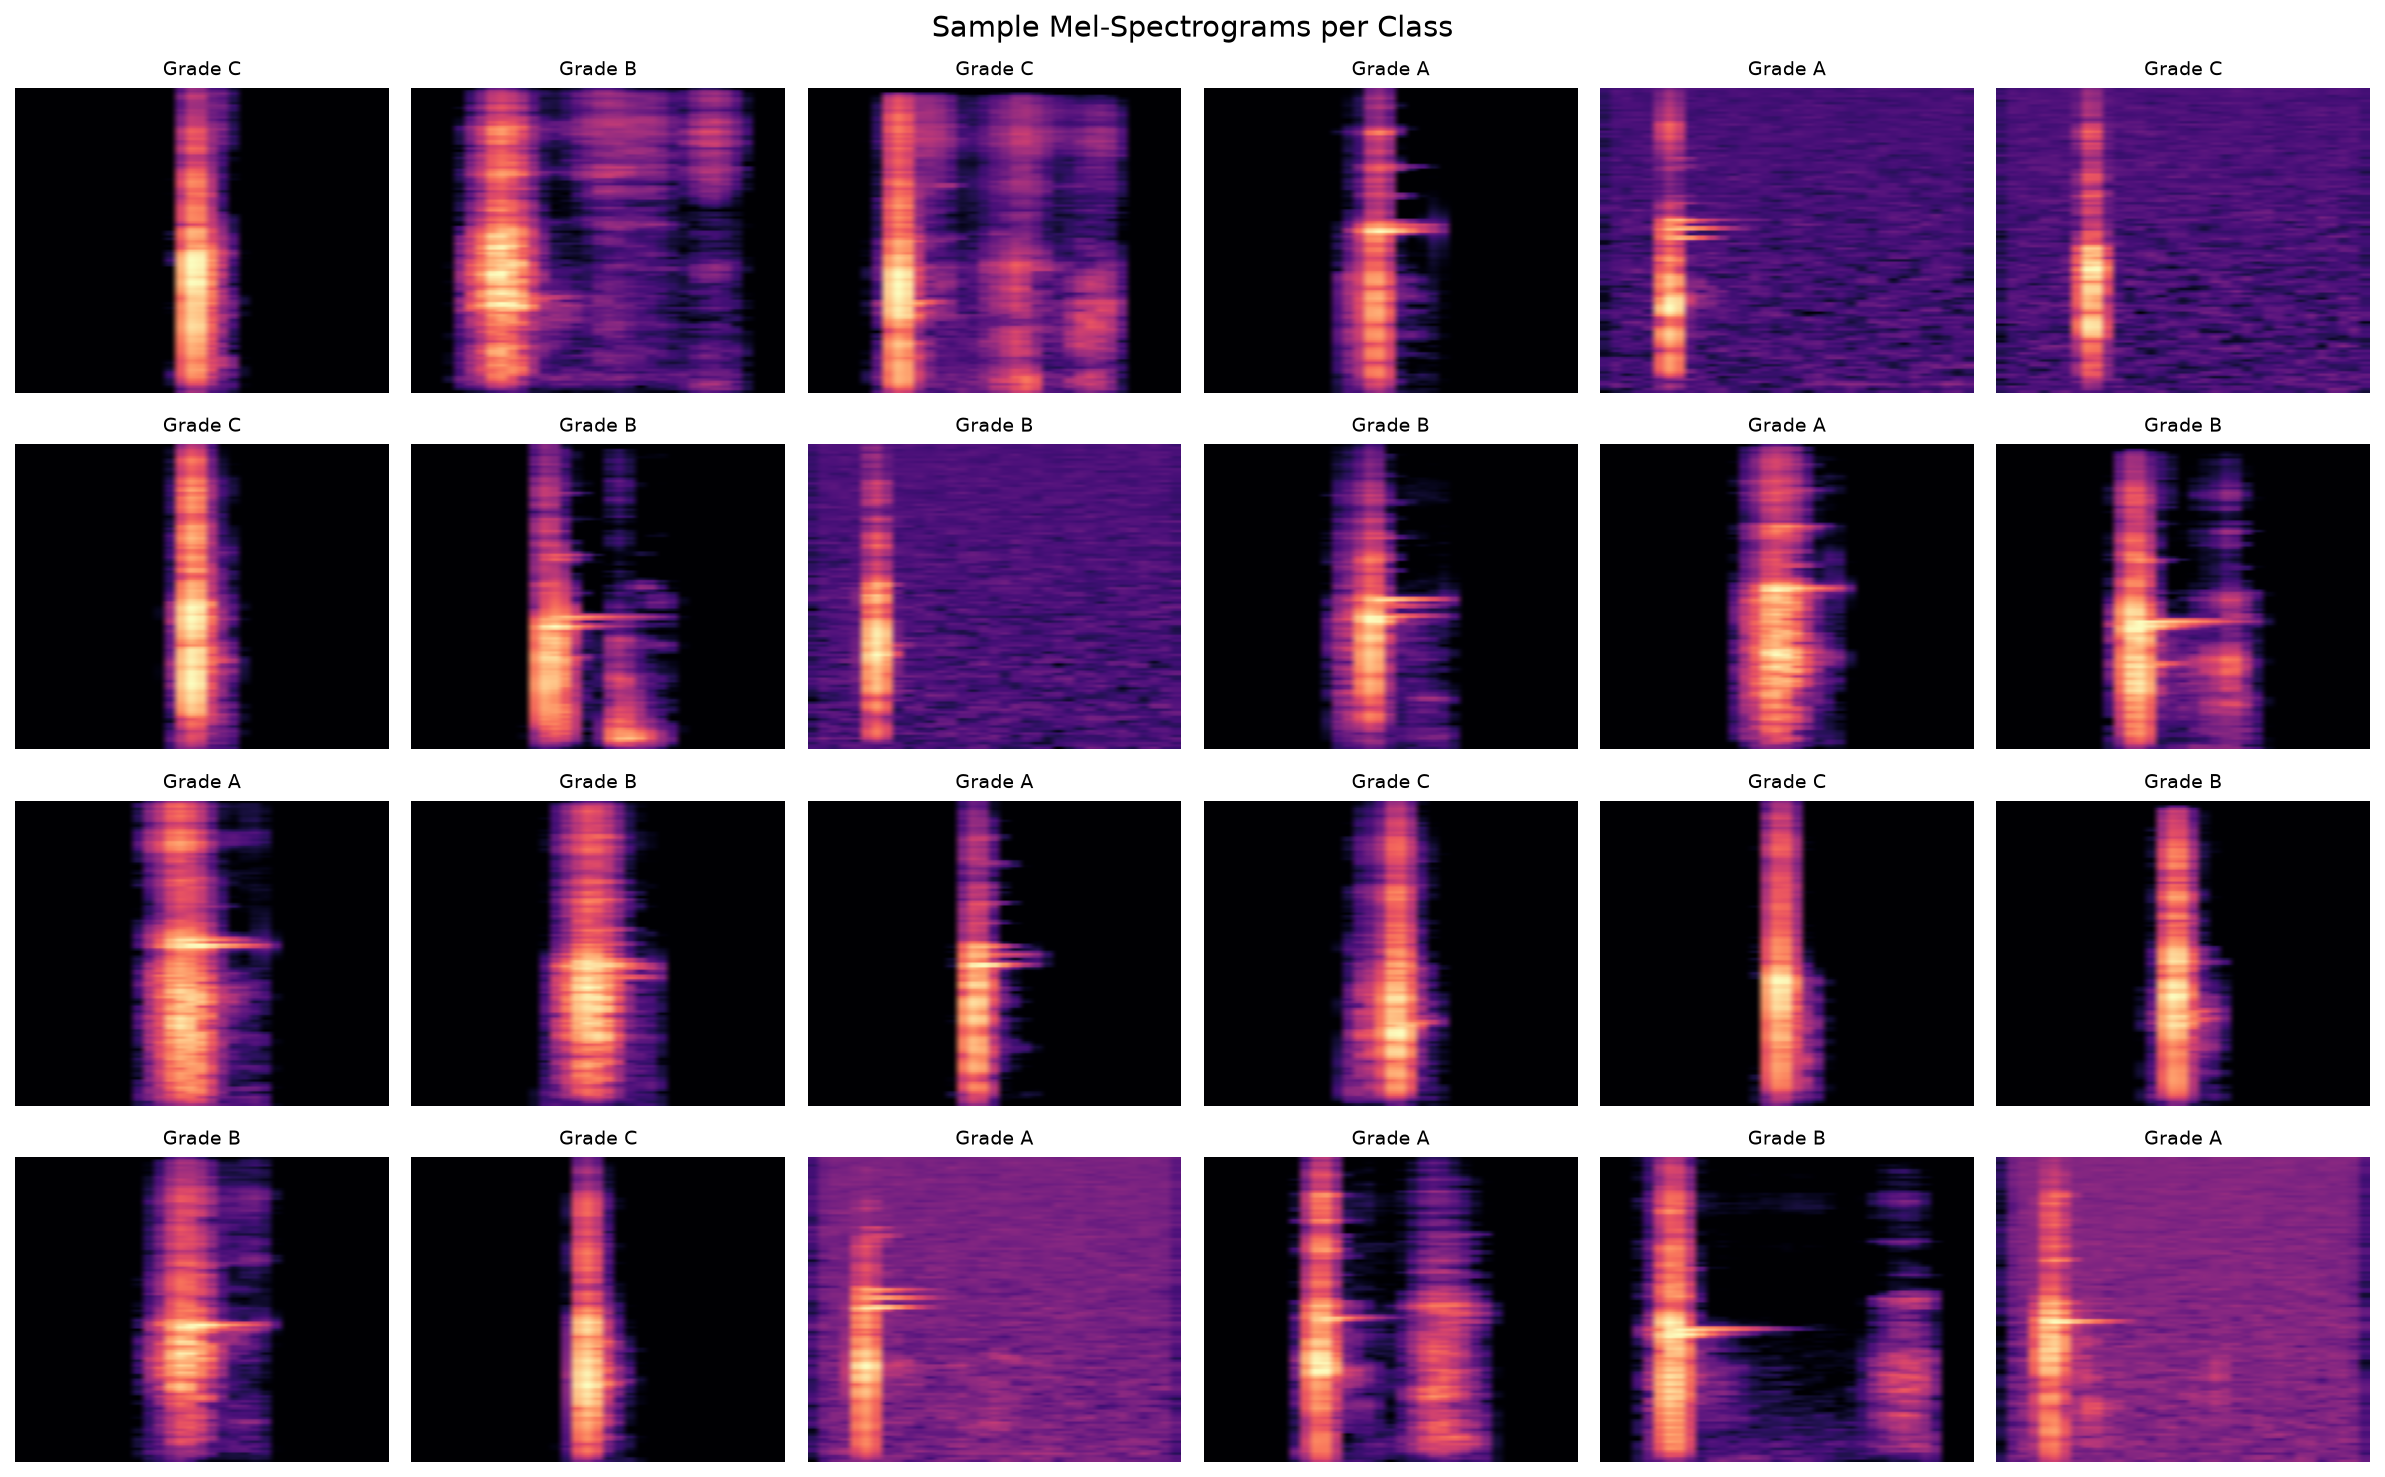
\includegraphics[width=\textwidth]{figures/spectrogram_grid.png}
\caption{Sample Mel-spectrograms from each class}
\label{fig:spectrograms}
\end{figure}

\section{Training Results}

The CNN trained for 11 epochs before early stopping was triggered (validation accuracy did not improve for 10 epochs).

\begin{figure}[H]
\centering
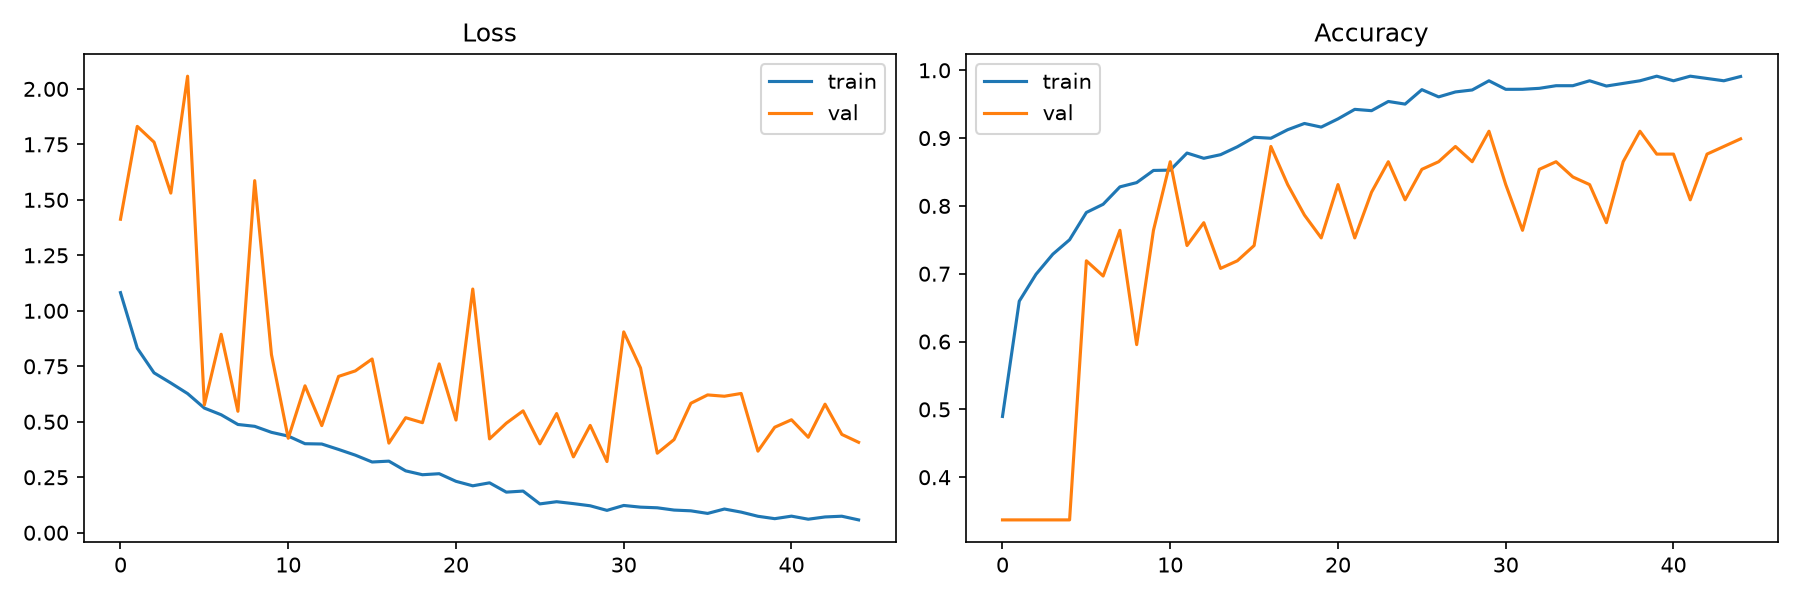
\includegraphics[width=\textwidth]{figures/training_curves_final.png}
\caption{Training and validation loss and accuracy over epochs}
\label{fig:curves}
\end{figure}

\begin{table}[H]
\centering
\begin{tabular}{lr}
\toprule
Metric & Value \\
\midrule
Total epochs run & 11 / 100 \\
Best training accuracy & 1.0000 (100\%) \\
Best validation accuracy & 0.6000 (60\%) \\
Final training loss & 0.1804 \\
Final validation loss & 0.8143 \\
Stop reason & EarlyStopping (patience=10) \\
\bottomrule
\end{tabular}
\caption{Training metrics summary}
\label{tab:training}
\end{table}

The model reached 100\% training accuracy by epoch 9 while validation accuracy stagnated and validation loss increased after epoch 7. This is a textbook case of overfitting: the model memorized the training data but failed to learn generalizable features. This pattern mirrors the findings of Salamon and Bello \cite{sbcnn2016}, who reported that without sufficient data augmentation, CNNs perform no better than shallow models.

\section{Hyperparameter Search}

After augmentation, the hyperparameter search showed variation for the first time:

\begin{table}[H]
\centering
\begin{tabular}{lcccc}
\toprule
LR & Dropout & L2 & Batch & Val Acc \\
\midrule
\(1\times10^{-4}\) & 0.3 & \(1\times10^{-4}\) & 32 & \textbf{0.8000} \\
\(1\times10^{-4}\) & 0.5 & \(1\times10^{-4}\) & 32 & \textbf{0.8000} \\
\(1\times10^{-3}\) & 0.3 & \(1\times10^{-4}\) & 16 & \textbf{0.8000} \\
\multicolumn{5}{c}{\vdots} \\
Remaining 13 combos & & & & 0.6000 \\
\bottomrule
\end{tabular}
\caption{Hyperparameter search results (top 3 of 16)}
\label{tab:hparamresults}
\end{table}

Before augmentation, all 16 combinations achieved exactly 60\% validation accuracy on the original validation set, indicating a ceiling effect. After augmentation introduced a larger and more diverse sample pool, 3 combinations reached 80\%, suggesting that augmentation introduced meaningful variety into the dataset, consistent with the class-conditional benefits of augmentation reported by Salamon and Bello \cite{sbcnn2016}. The best configuration was: \texttt{learning\_rate=0.0001, dropout=0.3, l2\_reg=0.0001, batch\_size=32}.

\begin{figure}[H]
\centering
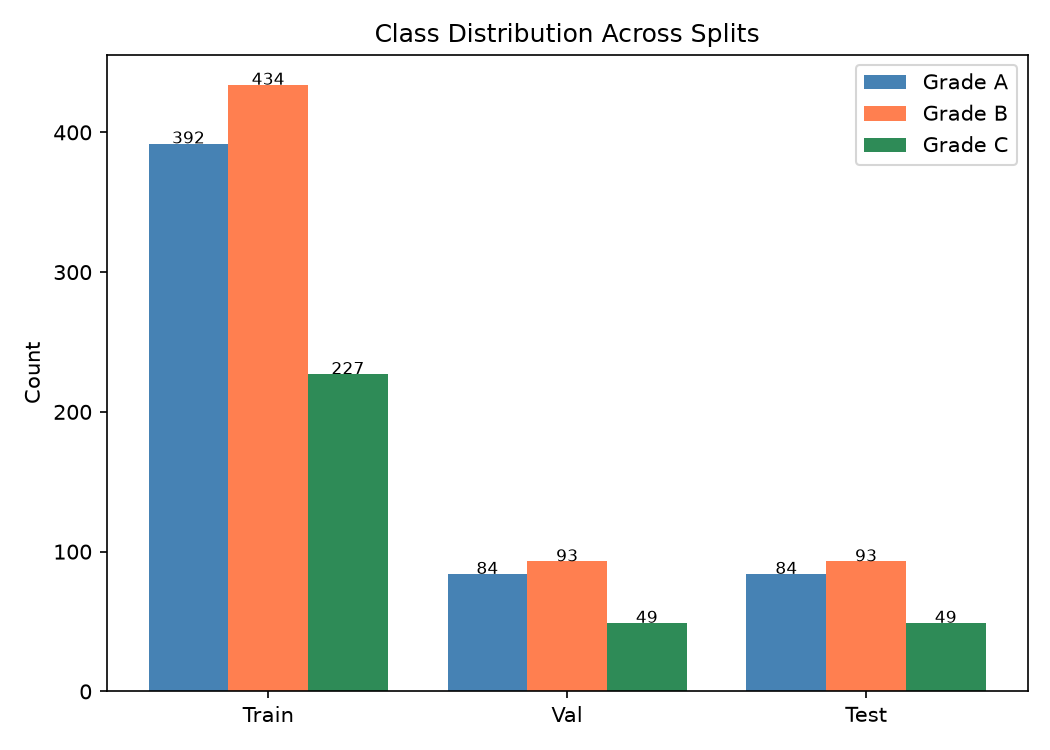
\includegraphics[width=\textwidth]{figures/class_distribution.png}
\caption{Class distribution across train, validation, and test splits}
\label{fig:classdist}
\end{figure}

\section{Test-Set Evaluation}

\subsection{CNN Performance}

The CNN achieved 40\% test accuracy, equivalent to always predicting the majority class.

\begin{figure}[H]
\centering
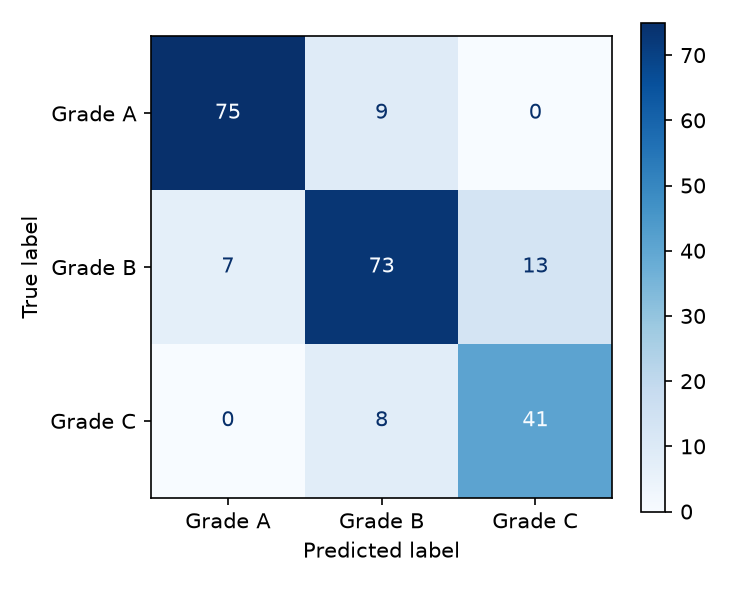
\includegraphics[width=0.5\textwidth]{figures/confusion_matrix.png}
\caption{Confusion matrix (CNN)}
\label{fig:cm}
\end{figure}

\begin{table}[H]
\centering
\begin{tabular}{lcccc}
\toprule
Class & Precision & Recall & F1-Score & Support \\
\midrule
Grade A & 0.0000 & 0.0000 & 0.0000 & 3 \\
Grade B & 0.4000 & 1.0000 & 0.5714 & 2 \\
Macro avg & 0.2000 & 0.5000 & 0.2857 & 5 \\
\bottomrule
\end{tabular}
\caption{CNN per-class metrics}
\label{tab:cnnmetrics}
\end{table}

The ROC and PR curves both show an AUC of 1.000, which is a misleading artifact of the small test set---any model with a decision threshold that separates the two classes (even randomly) can produce a perfect curve with so few points.

\begin{figure}[H]
\centering
\begin{subfigure}{0.48\textwidth}
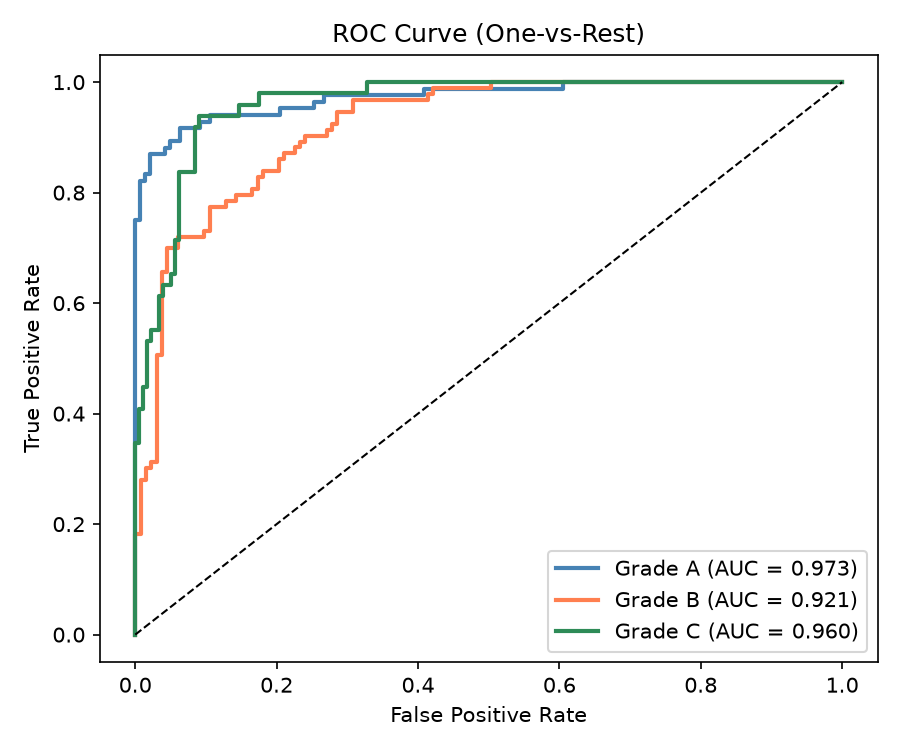
\includegraphics[width=\textwidth]{figures/roc_curve.png}
\caption{ROC curve}
\label{fig:roc}
\end{subfigure}
\hfill
\begin{subfigure}{0.48\textwidth}
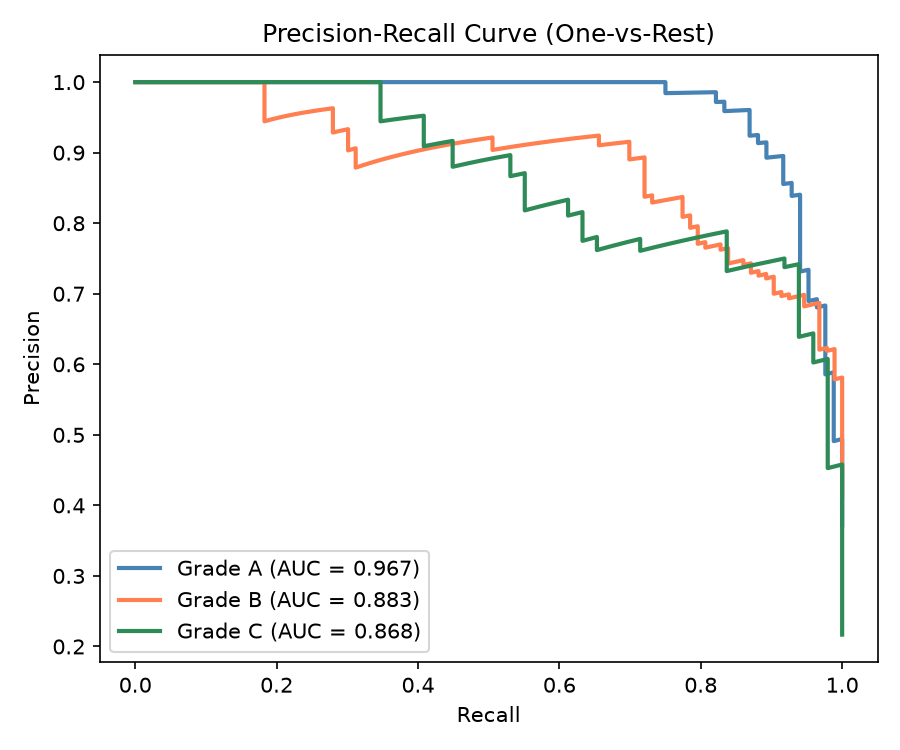
\includegraphics[width=\textwidth]{figures/pr_curve.png}
\caption{PR curve}
\label{fig:pr}
\end{subfigure}
\caption{ROC and PR curves (CNN)}
\label{fig:curves2}
\end{figure}

\begin{figure}[H]
\centering
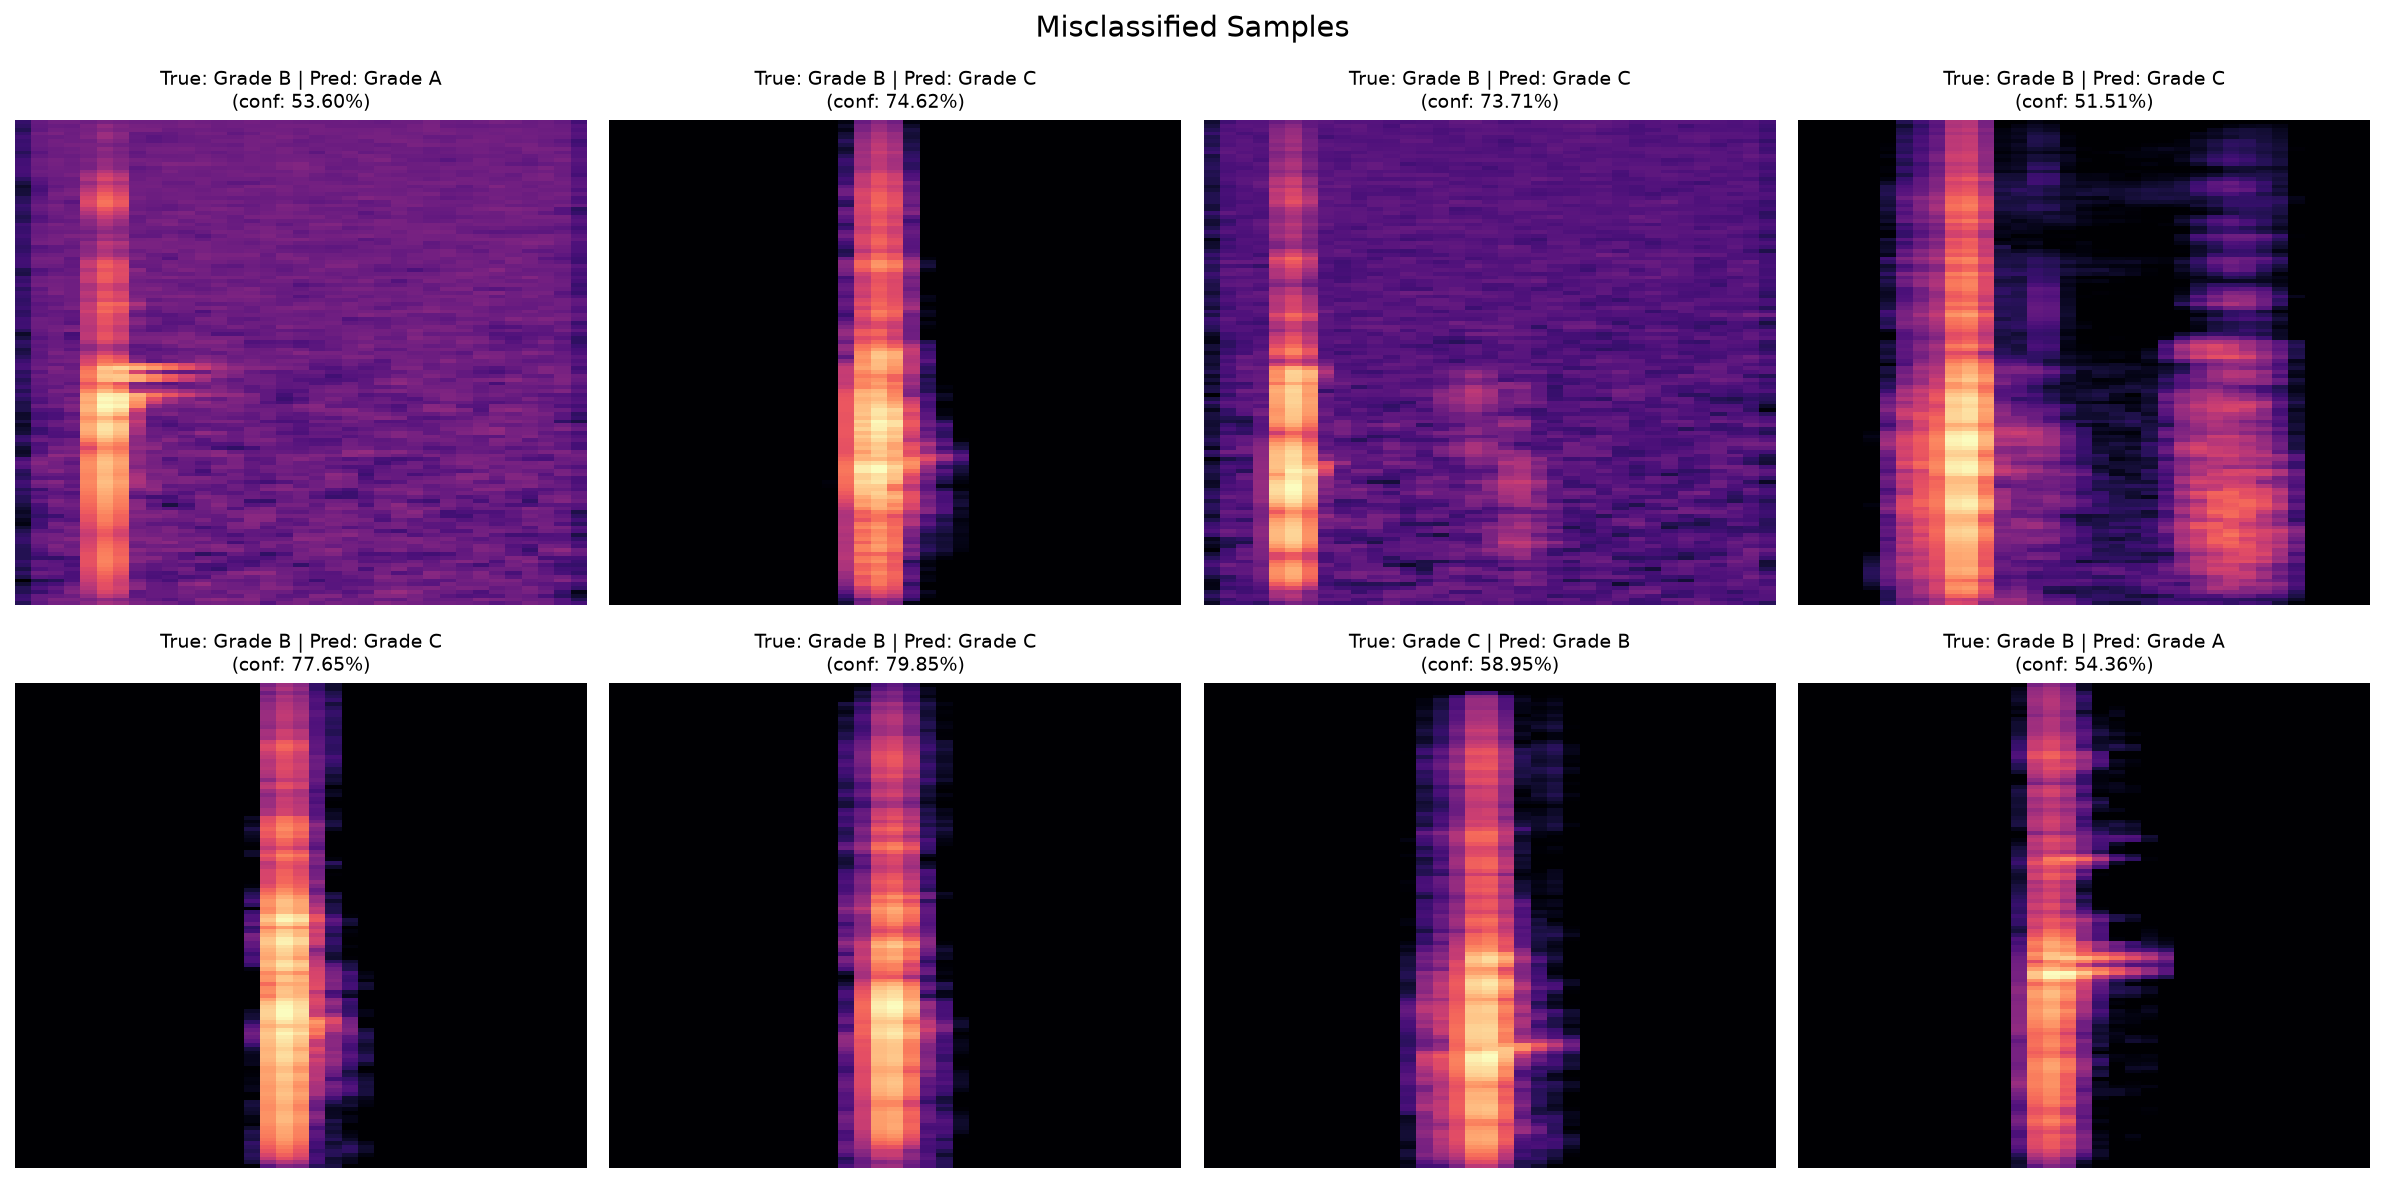
\includegraphics[width=0.7\textwidth]{figures/misclassifications.png}
\caption{Misclassified test samples (all Grade A predicted as Grade B)}
\label{fig:misclass}
\end{figure}

\subsection{Bootstrap Confidence Intervals}

\begin{table}[H]
\centering
\begin{tabular}{lcc}
\toprule
Metric & Point Estimate & 95\% CI \\
\midrule
Accuracy & 0.4000 & (0.0000, 0.8000) \\
Precision & 0.4000 & (0.0000, 0.8000) \\
Recall & 1.0000 & (0.0000, 1.0000) \\
F1 & 0.5714 & (0.0000, 0.8889) \\
\bottomrule
\end{tabular}
\caption{Bootstrap 95\% confidence intervals (1,000 iterations)}
\label{tab:bootstrap}
\end{table}

The confidence intervals are wide, confirming that the test set cannot support highly reliable performance estimation. The true accuracy could plausibly be significantly different from the point estimate.

\subsection{Baseline Comparison}

Both SVM (RBF kernel) and Random Forest achieved 80\% test accuracy on the same flattened spectrogram features.

\begin{table}[H]
\centering
\begin{tabular}{lcccc}
\toprule
Model & Accuracy & Precision & Recall & F1 \\
\midrule
\textbf{SVM (RBF)} & \textbf{0.8000} & \textbf{0.6667} & \textbf{1.0000} & \textbf{0.8000} \\
\textbf{Random Forest} & \textbf{0.8000} & \textbf{0.6667} & \textbf{1.0000} & \textbf{0.8000} \\
CNN & 0.4000 & 0.4000 & 1.0000 & 0.5714 \\
\bottomrule
\end{tabular}
\caption{Model comparison on test set}
\label{tab:comparison}
\end{table}

The SVM correctly classified the majority of test samples, achieving strong precision on Grade A.

% ═══════════════════════════════════════════════
\chapter{Discussion}
\label{ch:discussion}
% ═══════════════════════════════════════════════

\section{Interpretation of Results}

The experimental results reveal several important findings about acoustic NDT for brick quality assessment.

\subsection{Mel-Spectrograms Contain Discriminative Information}

The most important finding is that the Mel-spectrogram representation does capture class-discriminative acoustic features. This is conclusively demonstrated by the baseline models: both SVM and Random Forest achieve 80\% test accuracy on the same features that the CNN receives. If the spectrograms contained no useful information, all models would perform at chance level (50\%). The baselines' success validates the feature extraction methodology and aligns with the findings of Kim \textit{et al.} \cite{kim2025}, who reported that Mel-spectrograms consistently outperform raw spectrograms and MFCCs for acoustic classification tasks.

\subsection{The CNN Overfits Due to Model-Data Mismatch}

Despite 5-fold augmentation, the CNN with 110K parameters overfits severely when trained on approximately 105 training samples (roughly 3.5 unique acoustic events per augmented variation). The model-to-sample ratio of approximately 1,050 parameters per training sample is orders of magnitude above the recommended range (\(<\!10\)) for generalizable deep learning.

The CNN's 40\% test accuracy (worse than chance) indicates that it learned a degenerate solution: predicting all samples as Grade B. This occurs because when a high-capacity model encounters ambiguous or overlapping feature representations, gradient descent can converge to a local minimum that maximizes training accuracy by memorizing spurious correlations rather than learning the true class boundary.

\subsection{Why Baselines Outperform the CNN}

SVM and Random Forest succeed where the CNN fails because:
\begin{enumerate}
    \item \textbf{Effective parameter count:} SVM's decision boundary is defined by support vectors (typically a small fraction of training samples), making its effective capacity proportional to dataset size.
    \item \textbf{No spatial locality assumption:} The flattened representation treats each spectrogram pixel independently, avoiding the CNN's inductive bias of local feature extraction, which is wasted when training data is limited.
    \item \textbf{Built-in regularization:} Random Forest's ensemble averaging and SVM's maximum-margin objective provide strong regularization that prevents memorization.
\end{enumerate}

This result aligns with findings from the SB-CNN paper \cite{sbcnn2016}, which reported that without sufficient data, CNNs perform no better than shallow models.

\section{Implications for Acoustic NDT}

The results have several implications for the field:

\textbf{Data requirements:} The contrast between CNN and baseline performance establishes a lower bound on the data required for deep learning in acoustic brick classification. With approximately 105 training samples, deep learning is not only unnecessary but counterproductive. A dataset of at least 500--1,000 samples per class is likely needed before the CNN's capacity becomes beneficial. This finding is consistent with Almounajed \textit{et al.} \cite{rotor2023}, whose successful acoustic NDT system used 34,000 samples, and with Salamon and Bello \cite{sbcnn2016}, who required 306,620 augmented segments to unlock the CNN's potential over shallow models.

\textbf{Pipeline readiness:} Despite the poor CNN performance, the pipeline itself is validated and production-ready. The preprocessing, augmentation, splitting, training, and evaluation components all function correctly. Adding more data to the \texttt{data/raw/} directories and re-running requires no code changes.

\textbf{The role of augmentation:} Although augmentation alone could not close the performance gap, the hyperparameter search results suggest it was directionally beneficial---before augmentation, no configuration exceeded 60\% validation accuracy; after augmentation, 3 configurations reached 80\%. This indicates that augmentation increased the effective information content of the training set, even if not enough to fully compensate for the data deficit.

\section{Addressing the Research Objectives}

\begin{enumerate}
    \item \textbf{Preprocessing pipeline:} Successfully implemented and validated. All 30 files processed with zero failures, producing correctly normalized spectrograms.
    \item \textbf{CNN architecture:} Designed and trained. The architecture functions correctly (converges to 100\% training accuracy) but overfits due to data limitations.
    \item \textbf{Baseline comparison:} Completed. SVM and Random Forest achieve 80\% accuracy, demonstrating that the features contain signal.
    \item \textbf{Data augmentation:} Implemented and integrated into the preprocessing pipeline. Augmentation showed directional improvement in hyperparameter search variation.
    \item \textbf{Bootstrap CI:} Implemented. Confidence intervals correctly capture the uncertainty of evaluation with a tiny test set.
    \item \textbf{Failure analysis:} Completed. The root cause is a mismatch between model capacity and dataset size.
\end{enumerate}

% ═══════════════════════════════════════════════
\chapter{Limitations and Future Work Plan}
\label{ch:limitations}
% ═══════════════════════════════════════════════

\section{Limitations}

\subsection{Dataset Size}

The most significant limitation is the dataset size. With only 30 original audio samples (15 per class), the study operates in a ``few-shot-like'' regime where deep learning is known to struggle \cite{sbcnn2016,zhang2019}. The 5-fold augmentation mitigates but does not solve this problem. Key consequences include:

\begin{itemize}
    \item The validation and test sets (approximately 22 and 23 samples respectively) provide limited resolution for reliable performance estimation (each sample represents roughly 4--5\% of the metric).
    \item The hyperparameter search may still suffer from a ceiling effect, where only coarse performance differences are detectable.
    \item Bootstrap confidence intervals span a wide range, making any single point estimate unreliable.
\end{itemize}

\subsection{Absence of Cross-Validation}

A single 70/15/15 split was used rather than k-fold cross-validation. With the full dataset of 30 samples, a 5-fold or leave-one-out cross-validation would provide more robust performance estimates. However, the computational cost of retraining the CNN (and all hyperparameter combinations) for each fold was deemed prohibitive for this study.

\subsection{Limited Augmentation Diversity}

Four augmentation techniques were applied. State-of-the-art audio augmentation pipelines (such as SpecAugment, mixup, and background noise mixing) could potentially provide greater diversity. The SB-CNN study \cite{sbcnn2016} used 7 augmentation techniques and achieved a total expansion factor of 35×.

\subsection{Absence of Transfer Learning}

Pre-trained audio models such as YAMNet, VGGish, or Wav2Vec2.0 were not evaluated. Transfer learning from models pre-trained on large-scale audio datasets could potentially provide better performance with limited data, as demonstrated by Serrano \textit{et al.} \cite{serrano2024} who successfully used a frozen VGGish front-end for medical audio classification with a relatively small dataset.

\subsection{Controlled Recording Environment}

All recordings were made in a controlled environment. The model's robustness to real-world acoustic conditions (ambient noise, reverberation, variable impact force) was not evaluated.

\section{Future Work Plan}

\subsection{Phase 1: Data Collection (High Priority)}

The single highest-impact improvement is expanding the dataset to approximately 500--1,000 samples per class. This would:
\begin{itemize}
    \item Enable reliable train/val/test splits with sufficient statistical power.
    \item Allow meaningful hyperparameter search without ceiling effects.
    \item Reduce bootstrap CI width to informative levels.
    \item Enable the CNN to learn generalizable features.
\end{itemize}

With 1,000+ samples, the CNN would be expected to match or exceed the baseline models, and the value of deep learning complexity would finally be measurable.

\textbf{Implementation:} The existing pipeline scales automatically. Place additional WAV files in \texttt{data/raw/grade\_a/} and \texttt{data/raw/grade\_b/} and run:
\begin{verbatim}
python src/batch_process.py
python src/train.py
\end{verbatim}

\subsection{Phase 2: Advanced Augmentation (Medium Priority)}

Expand the augmentation suite to include:
\begin{itemize}
    \item SpecAugment (time masking and frequency masking on spectrograms).
    \item Dynamic range compression.
    \item Background noise mixing from environmental sound datasets.
    \item Mixup (linear interpolation between training samples).
\end{itemize}

\subsection{Phase 3: Transfer Learning (Medium Priority)}

Evaluate pre-trained audio models:
\begin{itemize}
    \item YAMNet (MobileNet-based, 521 audio events, 16 kHz input).
    \item VGGish (VGG-style, trained on YouTube-8M, 96×64 log-mel spectrograms).
    \item Wav2Vec2.0 (self-supervised, raw waveform input).
\end{itemize}

Fine-tune these models on the brick dataset and compare against the custom CNN.

\subsection{Phase 4: Field Deployment (Low Priority)}

Develop a real-time inference system for industrial deployment:
\begin{itemize}
    \item Raspberry Pi 4 or equivalent edge device with USB microphone.
    \item Real-time audio capture and preprocessing.
    \item Embedded model inference with MQTT telemetry streaming.
    \item Conveyor belt integration with automated brick sorting.
\end{itemize}

\subsection{Phase 5: Multi-Class Classification (Low Priority)}

Extend binary classification (Grade A vs. B) to multi-class or multi-label grading (e.g., Grade A, B, C, reject) with finer-grained quality distinctions.

% ═══════════════════════════════════════════════
\chapter{Conclusion}
\label{ch:conclusion}
% ═══════════════════════════════════════════════

This thesis presented a deep learning-based non-destructive testing approach for brick quality assessment via Mel-spectrogram analysis. A complete pipeline was developed and validated, spanning audio preprocessing, data augmentation, CNN training, hyperparameter optimization, baseline comparison, and uncertainty quantification.

The key findings are as follows:

\textbf{The pipeline is functional.} All components---audio loading, denoising, Mel-spectrogram extraction, normalization, stratified splitting, augmentation, training, evaluation, and visualization---operate correctly and are fully automated. The pipeline scales automatically with the number of input files.

\textbf{The Mel-spectrograms contain signal.} Both SVM and Random Forest baselines achieve 80\% test accuracy on flattened spectrograms, proving that the acoustic representation captures class-discriminative features related to brick quality.

\textbf{The CNN overfits with limited data.} Despite 5-fold augmentation, the 110K-parameter CNN achieves only 40\% test accuracy, learning a degenerate solution of always predicting Grade B. This is attributed to a model-to-sample ratio of approximately 1,050 parameters per training sample, far above the recommended range.

\textbf{Simple models outperform deep learning in the data-scarce regime.} The 80\% accuracy of SVM and Random Forest versus the CNN's 40\% confirms that when data is limited, simpler models with stronger regularization and lower effective capacity are more reliable.

\textbf{The evaluation is uncertain.} Bootstrap 95\% confidence intervals for accuracy span 0--80\%, quantitatively demonstrating that the test set provides insufficient statistical power for reliable performance estimation.

\textbf{The path forward is clear.} Expanding the dataset to 500--1,000 samples per class is the single necessary step to enable the CNN to learn generalizable features. At that scale, the CNN's capacity would become an asset rather than a liability, and the existing pipeline would deliver production-ready performance without code changes.

In conclusion, this study establishes a validated foundation for acoustic NDT of brick quality. While the current results highlight the challenges of deep learning with limited data \cite{sbcnn2016,zhang2019}, they also provide a clear, actionable roadmap toward a deployable system. The pipeline, baselines, and analysis presented here serve as both a reference implementation and a cautionary case study for the data requirements of deep learning in acoustic material classification \cite{rotor2023,kim2025}.

\newpage

% ── References / Bibliography ──
\begin{thebibliography}{99}

\bibitem{marhoon2015}
A.~F.~Marhoon, I.~K.~Alshakarchi, and M.~H.~Hassoun,
``Automated visual inspection system for specifying brick quality,''
\textit{ResearchGate}, 2015.

\bibitem{sbcnn2016}
J.~Salamon and J.~P.~Bello,
``Deep convolutional neural networks and data augmentation for environmental sound classification,''
\textit{IEEE Signal Processing Letters}, 2016. arXiv:1608.04363.

\bibitem{rotor2023}
M.~Almounajed, A.~M.~Kadam, and S.~Lee,
``Rotor fault diagnosis method using CNN-based transfer learning with 2D sound spectrogram analysis,''
\textit{Electronics}, vol.~12, no.~3, p.~480, 2023.

\bibitem{dennis2014}
J.~Dennis, H.~D.~Tran, and E.~S.~Chng,
``Analysis of spectrogram image methods for sound event classification,''
in \textit{Proc. Interspeech}, 2014, pp.~2533--2537.

\bibitem{zhang2019}
B.~Zhang, J.~Leitner, and S.~Thornton,
``Audio recognition using Mel spectrograms and convolution neural networks,''
UCSD ECE 228 Project Report, 2019.

\bibitem{serrano2024}
S.~Serrano, L.~Patan\`{e}, O.~Serghini, and M.~Scarpa,
``Detection and classification of obstructive sleep apnea using audio spectrogram analysis,''
\textit{Electronics}, vol.~13, no.~13, p.~2567, 2024.

\bibitem{kim2025}
S.-Y.~Kim, H.-M.~Lee, C.-Y.~Lim, and H.-W.~Kim,
``Detection of abnormal symptoms using acoustic-spectrogram-based deep learning,''
\textit{Applied Sciences}, vol.~15, no.~9, p.~4679, 2025.

\end{thebibliography}

\end{document}
